\documentclass[12pt,a4paper]{article}
\usepackage[T1]{fontenc}
\usepackage[margin=1 cm]{geometry}
\usepackage{amsmath}
\usepackage{graphicx}
\title{Study about the conductivity equation}
\author{A R Bathri Narayanan P0211501\\Ranya Sharma P02115}
\date{}
\begin{document}
	\maketitle
	\par\noindent\rule{\textwidth}{0.4pt}
	We have the conductivity equation derived in class
	\[\sigma = \sigma_0 e^{\frac{-\Delta}{kT}}\]
	Taking a derivative of that with respect to temperature
	\[\frac{d\sigma}{dT}=\sigma_0e^{\frac{-\Delta}{kT}}\frac{\Delta}{kT^2}\]
	Means the function will be at it's extrema at T $\rightarrow$ 0 or T $\rightarrow \infty$ (T$\neq$0 as it will violate the third law of thermodynamics)
	Taking the second derivative to check for inflection points
	\begin{align*}
		\frac{d^2\sigma}{dT^2}=\sigma_0\frac{\Delta^2}{k^2T^4}e^{\frac{-\Delta}{kT}}-2\sigma_0e^{\frac{-\Delta}{kT}}\frac{\Delta}{kT^3}
	\end{align*}
	Finding the inflection points
	\[\sigma_0\frac{\Delta^2}{k^2T^4}e^{\frac{-\Delta}{kT}}=2\sigma_0e^{\frac{-\Delta}{kT}}\frac{\Delta}{kT^3}\]
	\[\frac{\Delta}{2kT}=1 \text{ or } T = \frac{\Delta}{2k}\]
	 But as the function is a monotonically increasing function, this should increase, stop and still increase but at a slower rate.
	 But if we try to find the order of inflection point, taking $\Delta$ to be around 0.05-0.5 eV, meaning T should be around $(0.29-2.9) \times 10^{3} K.$\\
	 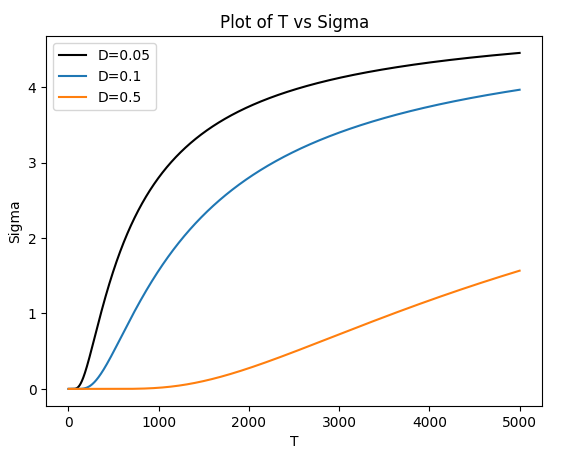
\includegraphics[width=10 cm]{sigma1.png}
	  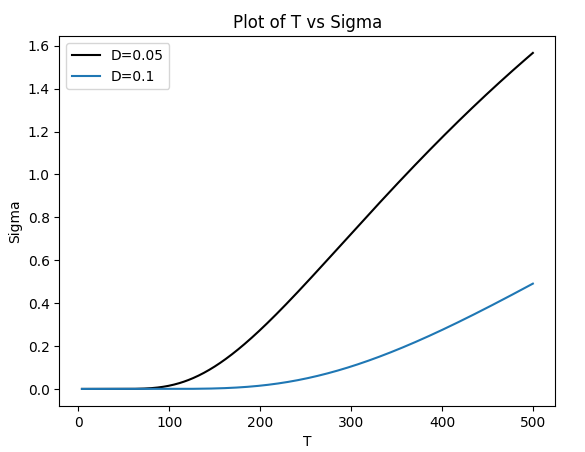
\includegraphics[width=10 cm]{sigma2.png}
	  Graphs for reference (Taking $\sigma_0$=1 for ease), note that due to resolution, the graph appears to be touching 0, but it starts from 4K, the temperature of liquid Helium.\\
\newpage 
Now we take $\Delta$'s range from 0.01 to 0.1 and try plotting the graphs for $\sigma$ vs T, $\frac{d\sigma}{dT}$ and $\frac{d^2\sigma}{dT^2}$
\begin{center}
	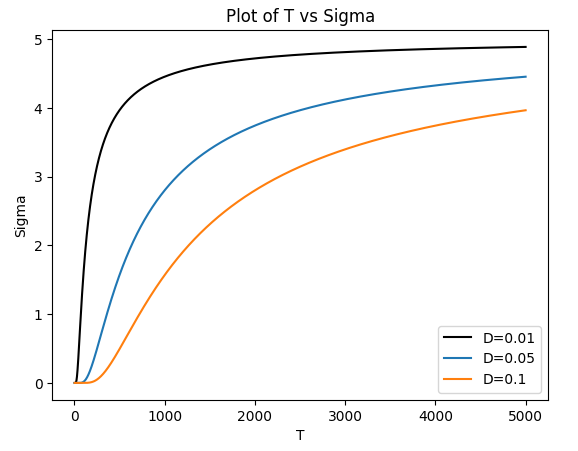
\includegraphics[width=10 cm]{sigma3.png}\\
		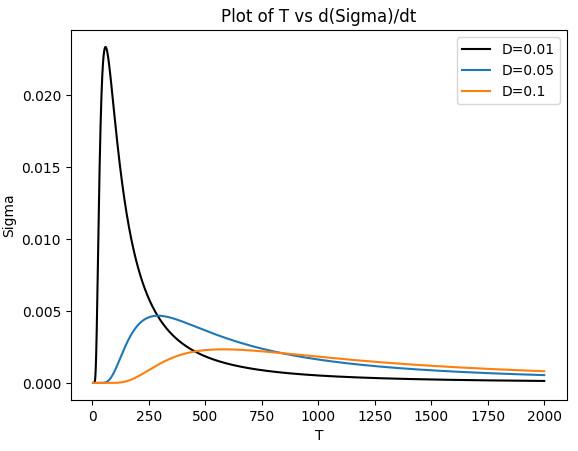
\includegraphics[width=10 cm]{sigma4.png}\\
			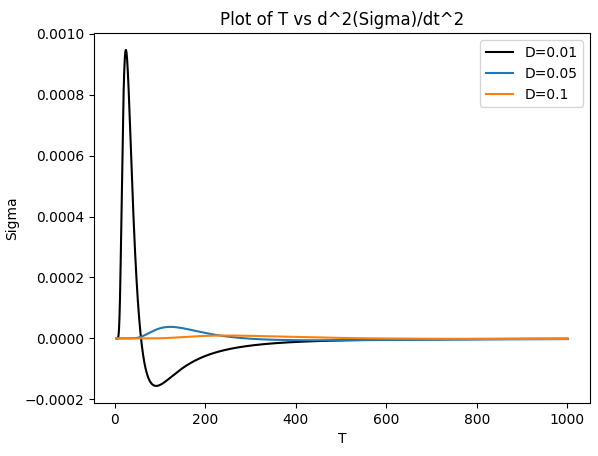
\includegraphics[width=10 cm]{sigma5.png}
\end{center}
The inflection points are respectively at 58.0 K, 290.1 K and 580.2 K as we increase $\Delta$ from 0.01 to 0.1, with 290.1 K at 0.05.
\section*{Appendix}
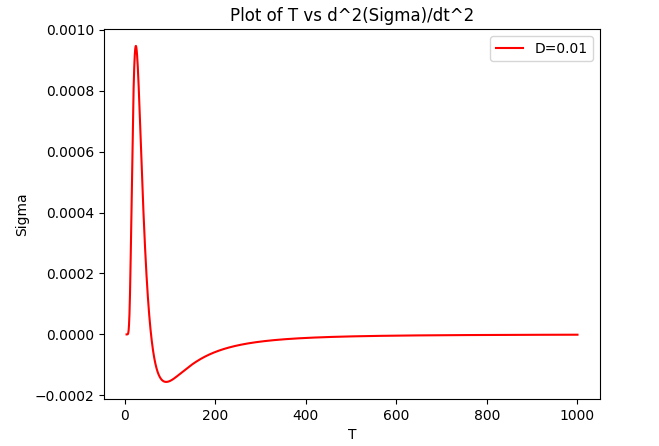
\includegraphics[width=6.5 cm]{sigma6.png}
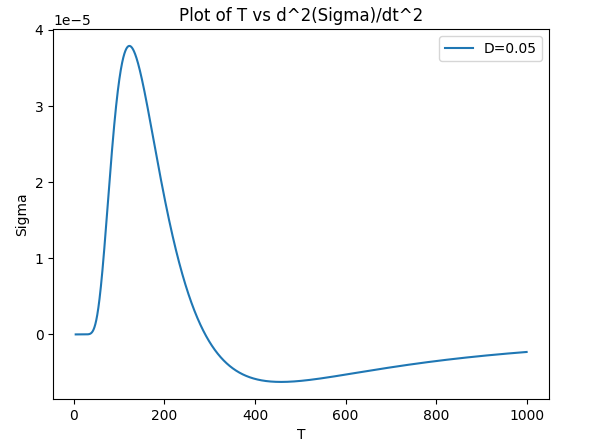
\includegraphics[width=6.5 cm]{sigma7.png}
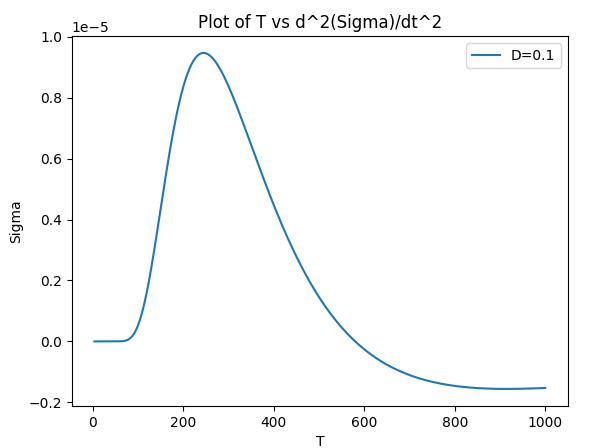
\includegraphics[width=6.5 cm]{sigma8.png}\\
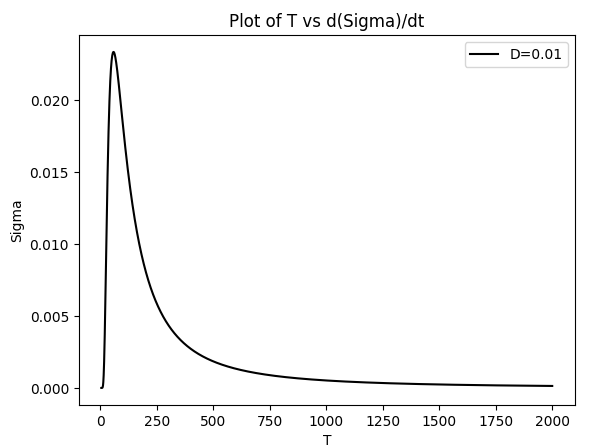
\includegraphics[width=6.5 cm]{sigma9.png}
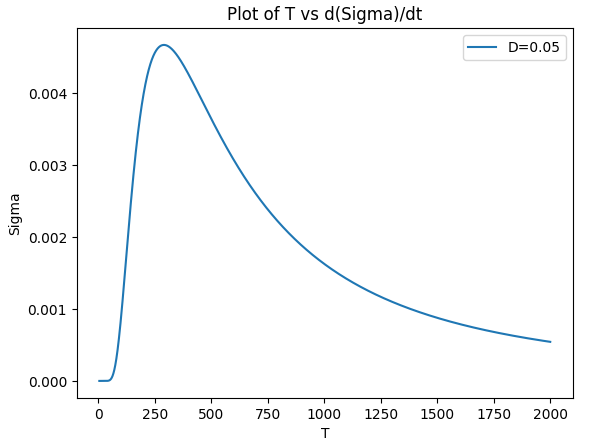
\includegraphics[width=6.5 cm]{sigma10.png}
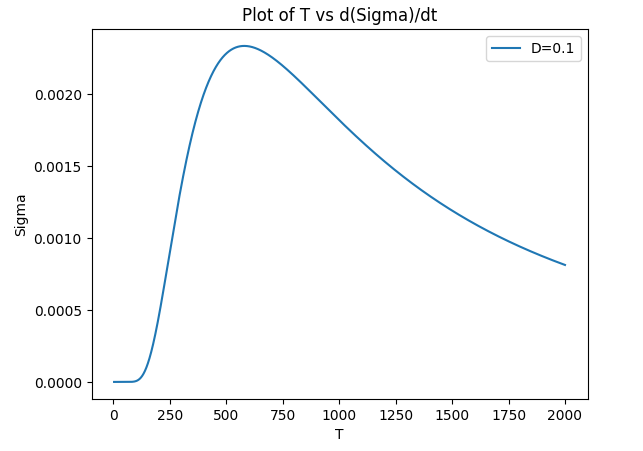
\includegraphics[width=6.5 cm]{sigma11.png}\\
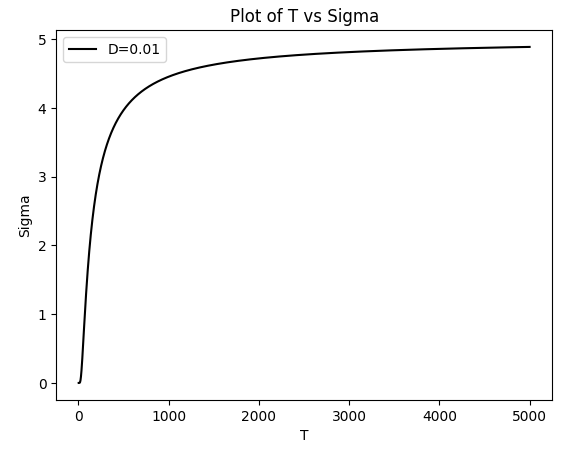
\includegraphics[width=6.5 cm]{sigma12.png}
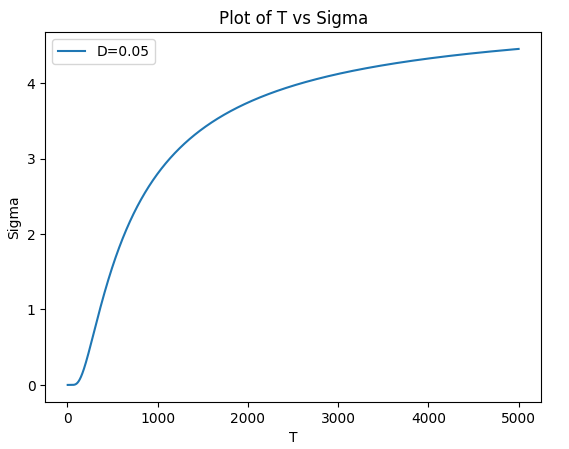
\includegraphics[width=6.5 cm]{sigma13.png}
\includegraphics[width=6.5 cm]{sigma14.png}\\

\end{document}